% !TEX program = lualatex
\documentclass[a4paper,11pt]{ltjsarticle}

% LuaLaTeX用日本語設定
\usepackage{luatexja}
\usepackage{luatexja-fontspec}
\usepackage[ipaex]{luatexja-preset}

% 数学パッケージ
\usepackage{amsmath, amssymb, amsthm}
\usepackage{mathtools}

% 図式用パッケージ
\usepackage{tikz}
\usepackage{tikz-cd}
\usetikzlibrary{positioning, arrows.meta, calc, shapes.geometric, fit, backgrounds}

% その他
\usepackage{hyperref}
\usepackage{enumerate}
\usepackage{tcolorbox}
\tcbuselibrary{theorems, breakable}

% 定理環境
\theoremstyle{definition}
\newtheorem{definition}{定義}[section]
\newtheorem{theorem}[definition]{定理}
\newtheorem{lemma}[definition]{補題}
\newtheorem{proposition}[definition]{命題}
\newtheorem{example}[definition]{例}
\newtheorem{remark}[definition]{注意}
\newtheorem{corollary}[definition]{系}

% マクロ
\newcommand{\rank}{\operatorname{rank}}
\newcommand{\layer}{\operatorname{layer}}
\newcommand{\minLayer}{\operatorname{minLayer}}
\newcommand{\step}{\operatorname{step}}
\newcommand{\iter}{\operatorname{iter}}
\newcommand{\WithTop}{\operatorname{WithTop}}

% タイトル情報
\title{Ranked構造の必須例カタログ\\
{\large 5つの典型例による数学的解説}}
\author{%
  Leanファイル生成: Codex (OpenAI)\\
  TeXファイル生成: Claude Code (Anthropic)
}
\date{\today}

\begin{document}

\maketitle

\begin{abstract}
本稿では、階層構造（Ranked構造）の5つの典型的な例について詳述する。
リストの長さ、有限集合の濃度、多項式の次数、整数の絶対値、そして拡張演算子の反復回数という、
それぞれ異なる数学的文脈における階層化の手法を形式的に定義し、その性質を考察する。
全ての定義と定理はLean 4において形式的に検証されている。
\end{abstract}

\tableofcontents

\section{導入}

\subsection{Ranked構造とは}

数学的対象を「階層」や「次数」によって分類することは、様々な分野で基本的な手法である。
本稿で扱うRanked構造は、この直観を形式化したものである。

\begin{definition}[Ranked構造]
\label{def:ranked}
型 $\alpha$ 上の順序型 $I$ によるRanked構造とは、rank関数 $\rank : \alpha \to I$ を指定することである。
各順序 $i \in I$ に対して、層（layer）を次のように定義する：
\[
\layer(i) = \{ x \in \alpha \mid \rank(x) \leq i \}
\]
\end{definition}

\subsection{本稿の構成}

本稿では以下の5つの例を扱う：

\begin{enumerate}
\item \textbf{ListLength}（\S\ref{sec:listlength}）：リストの長さ
\item \textbf{FinsetCard}（\S\ref{sec:finsetcard}）：有限集合の濃度
\item \textbf{PolyDegree}（\S\ref{sec:polydegree}）：多項式の次数
\item \textbf{IntAbs}（\S\ref{sec:intabs}）：整数の絶対値
\item \textbf{ClosureIteration}（\S\ref{sec:closure}）：閉包演算の反復回数
\end{enumerate}

これらの例は、計算的な対象（リスト）、組合せ論的な対象（有限集合）、代数的な対象（多項式・整数）、
そして動的な対象（反復演算）という、多様な数学的文脈をカバーしている。

\begin{figure}[h]
\centering
\begin{tikzpicture}[
  node distance=2cm,
  box/.style={rectangle, draw, minimum width=2.5cm, minimum height=1cm, align=center},
  arrow/.style={-Stealth, thick}
]
  \node[box] (list) {List\\(長さ)};
  \node[box, right=of list] (finset) {Finset\\(濃度)};
  \node[box, below=of list] (poly) {Polynomial\\(次数)};
  \node[box, below=of finset] (int) {Int\\(絶対値)};
  \node[box, below right=1cm and 0.5cm of poly] (closure) {Set\\(反復回数)};

  \draw[arrow] (list) -- node[above] {\small toFinset} (finset);

  \node[above=0.5cm of list, xshift=1cm] {\textbf{計算的}};
  \node[above=0.5cm of poly, xshift=1cm] {\textbf{代数的}};
  \node[left=0.5cm of closure] {\textbf{動的}};
\end{tikzpicture}
\caption{5つの例の分類と関係}
\label{fig:overview}
\end{figure}

\section{ListLength - リストの長さ}
\label{sec:listlength}

\subsection{定義}

リストは最も基本的な計算的データ構造の一つである。その長さは自然な階層化を与える。

\begin{definition}[リストのRanked構造]
\label{def:list-ranked}
型 $\alpha$ 上のリスト $\text{List}\,\alpha$ に対して：
\begin{itemize}
\item $\rank(l) = |l|$（リストの長さ）
\item $\layer(n) = \{ l \in \text{List}\,\alpha \mid |l| \leq n \}$
\end{itemize}
\end{definition}

\subsection{基本性質}

\begin{proposition}[層の単調性]
$m \leq n$ ならば $\layer(m) \subseteq \layer(n)$
\end{proposition}

\begin{proposition}[特殊な要素]
\begin{itemize}
\item 空リスト $[]$ は $\layer(0)$ に属する
\item 任意のリスト $l$ は $\layer(|l|)$ に属する
\end{itemize}
\end{proposition}

\subsection{具体例}

\begin{table}[h]
\centering
\begin{tabular}{|c|c|c|}
\hline
リスト $l$ & $\rank(l)$ & 最小層 \\
\hline
$[]$ & $0$ & $\layer(0)$ \\
$[1]$ & $1$ & $\layer(1)$ \\
$[1, 2]$ & $2$ & $\layer(2)$ \\
$[1, 2, 3]$ & $3$ & $\layer(3)$ \\
$[1, 2, 3, 4, 5]$ & $5$ & $\layer(5)$ \\
\hline
\end{tabular}
\caption{リストの例}
\label{tab:list-examples}
\end{table}

\section{FinsetCard - 有限集合の濃度}
\label{sec:finsetcard}

\subsection{定義}

有限集合の濃度（要素数）は組合せ論における基本的な不変量である。

\begin{definition}[有限集合のRanked構造]
\label{def:finset-ranked}
型 $\alpha$ 上の有限集合 $\text{Finset}\,\alpha$ に対して：
\begin{itemize}
\item $\rank(S) = |S|$（集合の濃度）
\item $\layer(n) = \{ S \in \text{Finset}\,\alpha \mid |S| \leq n \}$
\end{itemize}
\end{definition}

\subsection{重要な性質}

\begin{theorem}[部分集合の性質]
$S \subseteq T$ ならば $\rank(S) \leq \rank(T)$
\end{theorem}

\begin{proposition}[特殊な要素]
\begin{itemize}
\item 空集合 $\emptyset$ は $\layer(0)$ に属する
\item 単元集合 $\{x\}$ は $\layer(1)$ に属する
\end{itemize}
\end{proposition}

\subsection{ListからFinsetへの準同型}

\begin{definition}[RankHomLe]
リストから有限集合への変換 $\text{toFinset} : \text{List}\,\alpha \to \text{Finset}\,\alpha$ は
rank準同型（RankHomLe）を定める：
\[
\rank(\text{toFinset}(l)) \leq \rank(l)
\]
\end{definition}

これは重複要素の除去により濃度が減少することを反映している。

\begin{figure}[h]
\centering
\begin{tikzcd}[column sep=large]
\text{List}\,\alpha \arrow[r, "\text{toFinset}"] \arrow[d, "\rank"']
& \text{Finset}\,\alpha \arrow[d, "\rank"] \\
\mathbb{N} \arrow[r, "\text{id}"', "\leq"]
& \mathbb{N}
\end{tikzcd}
\caption{ListからFinsetへのRankHomLe}
\label{fig:rankhomle}
\end{figure}

\section{PolyDegree - 多項式の次数}
\label{sec:polydegree}

\subsection{定義}

多項式環における次数は、代数学において最も基本的な不変量の一つである。

\begin{definition}[多項式のRanked構造]
\label{def:poly-ranked}
半環 $R$ 上の多項式環 $R[X]$ に対して：
\begin{itemize}
\item $\rank(p) = \deg p$（多項式の次数、Leanでは $\text{natDegree}$）
\item $\layer(n) = \{ p \in R[X] \mid \deg p \leq n \}$
\end{itemize}
\end{definition}

\begin{tcolorbox}[colback=blue!5!white, colframe=blue!75!black, title=重要な注意]
Mathlibでは $\text{natDegree}(0) = 0$ と定義されている。
したがって $\layer(0)$ にはゼロ多項式と全ての定数多項式が含まれる。
\end{tcolorbox}

\subsection{代数的性質}

\begin{proposition}[加法に関する性質]
任意の $p, q \in R[X]$ に対して、
\[
\rank(p + q) \leq \max\{\rank(p), \rank(q)\}
\]
\end{proposition}

\begin{corollary}[層の加法閉性]
各層 $\layer(n)$ は加法に関して閉じている。
\end{corollary}

\subsection{層の特徴付け}

\begin{theorem}[第0層]
\[
\layer(0) = \{ p \in R[X] \mid \exists c \in R,\, p = c \text{ または } p = 0 \}
\]
すなわち、$\layer(0)$ は定数多項式全体である。
\end{theorem}

\begin{figure}[h]
\centering
\begin{tikzpicture}[scale=1.1]
  % Layer 0
  \draw[thick, fill=green!20] (0,0) ellipse (1.2 and 0.6);
  \node at (0,0) {\small $\layer(0)$};
  \node[below, font=\tiny] at (0,-0.4) {定数};

  % Layer 1
  \draw[thick, fill=green!15] (0,0) ellipse (2 and 1);
  \node at (0,-0.8) {\small $\layer(1)$};

  % Layer 2
  \draw[thick, fill=green!10] (0,0) ellipse (2.8 and 1.4);
  \node at (0,-1.2) {\small $\layer(2)$};

  % Layer n
  \draw[thick, fill=green!5] (0,0) ellipse (3.6 and 1.8);
  \node at (0,-1.6) {\small $\layer(n)$};

  % Examples
  \node at (0, 0.2) {\small $0, c$};
  \node at (1.3, 0.2) {\small $X$};
  \node at (2.2, 0.2) {\small $X^2$};
\end{tikzpicture}
\caption{多項式環の層構造}
\label{fig:poly-layers}
\end{figure}

\section{IntAbs - 整数の絶対値}
\label{sec:intabs}

\subsection{定義}

整数の絶対値は、原点からの距離を測る自然な関数である。

\begin{definition}[整数のRanked構造]
\label{def:int-ranked}
整数 $\mathbb{Z}$ に対して：
\begin{itemize}
\item $\rank(z) = |z|$（絶対値）
\item $\layer(n) = \{ z \in \mathbb{Z} \mid |z| \leq n \} = [-n, n] \cap \mathbb{Z}$
\end{itemize}
\end{definition}

\subsection{幾何的解釈}

整数を原点からの距離で階層化すると考えることができる：

\begin{itemize}
\item $\layer(0) = \{0\}$（原点のみ）
\item $\layer(1) = \{-1, 0, 1\}$（原点と隣接点）
\item $\layer(n) = \{-n, \ldots, -1, 0, 1, \ldots, n\}$（原点中心の区間）
\end{itemize}

\begin{figure}[h]
\centering
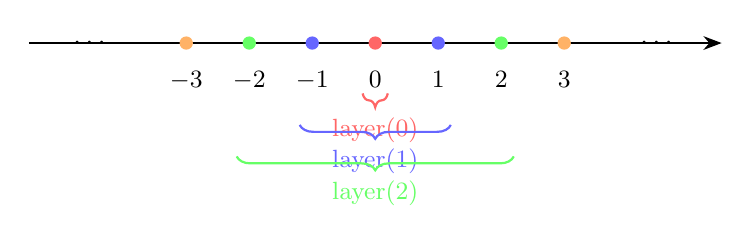
\begin{tikzpicture}[scale=0.8]
  % Number line
  \draw[thick, -Stealth] (-5.5, 0) -- (5.5, 0);

  % Layer 0
  \fill[red!60] (0,0) circle (3pt);
  \node[below] at (0,-0.3) {\small $0$};
  \draw[red!60, thick, decorate, decoration={brace, amplitude=5pt, mirror}]
    (-0.2,-0.8) -- (0.2,-0.8) node[midway, below=5pt] {\small $\layer(0)$};

  % Layer 1
  \fill[blue!60] (-1,0) circle (3pt);
  \fill[blue!60] (1,0) circle (3pt);
  \node[below] at (-1,-0.3) {\small $-1$};
  \node[below] at (1,-0.3) {\small $1$};
  \draw[blue!60, thick, decorate, decoration={brace, amplitude=5pt, mirror}]
    (-1.2,-1.3) -- (1.2,-1.3) node[midway, below=5pt] {\small $\layer(1)$};

  % Layer 2
  \fill[green!60] (-2,0) circle (3pt);
  \fill[green!60] (2,0) circle (3pt);
  \node[below] at (-2,-0.3) {\small $-2$};
  \node[below] at (2,-0.3) {\small $2$};
  \draw[green!60, thick, decorate, decoration={brace, amplitude=5pt, mirror}]
    (-2.2,-1.8) -- (2.2,-1.8) node[midway, below=5pt] {\small $\layer(2)$};

  % Layer 3
  \fill[orange!60] (-3,0) circle (3pt);
  \fill[orange!60] (3,0) circle (3pt);
  \node[below] at (-3,-0.3) {\small $-3$};
  \node[below] at (3,-0.3) {\small $3$};

  % Dots
  \node at (-4.5, 0) {$\cdots$};
  \node at (4.5, 0) {$\cdots$};
\end{tikzpicture}
\caption{整数の層構造（数直線上の表現）}
\label{fig:int-layers}
\end{figure}

\subsection{対称性と三角不等式}

\begin{proposition}[対称性]
任意の $z \in \mathbb{Z}$ に対して $\rank(-z) = \rank(z)$
\end{proposition}

\begin{proposition}[三角不等式]
任意の $z_1, z_2 \in \mathbb{Z}$ に対して
\[
\rank(z_1 + z_2) \leq \rank(z_1) + \rank(z_2)
\]
\end{proposition}

\subsection{層の非閉性}

ListやPolynomialとは異なり、整数の層は代数演算で閉じていない：

\begin{example}[加法非閉性]
$1, 1 \in \layer(1)$ だが $1 + 1 = 2 \notin \layer(1)$
\end{example}

\begin{example}[乗法非閉性]
$2, 2 \in \layer(2)$ だが $2 \times 2 = 4 \notin \layer(2)$
\end{example}

\section{ClosureIteration - 閉包演算の反復}
\label{sec:closure}

\subsection{拡張演算子}

前の4つの例とは異なり、この例では動的な過程（反復）を階層化する。

\begin{definition}[拡張演算子]
型 $X$ 上の拡張演算子とは、関数 $\step : \mathcal{P}(X) \to \mathcal{P}(X)$ であって以下を満たすもの：
\begin{enumerate}
\item \textbf{拡張性}：$S \subseteq \step(S)$
\item \textbf{単調性}：$S \subseteq T \implies \step(S) \subseteq \step(T)$
\end{enumerate}
\end{definition}

\begin{remark}
冪等性（$\step(\step(S)) = \step(S)$）は仮定しない。冪等性を仮定すると、
全ての集合が高々1ステップで安定化してしまい、興味深い例が得られない。
\end{remark}

\subsection{反復とrank}

\begin{definition}[反復]
$n$ 回の反復を $\iter^n(S)$ で表す：
\[
\iter^0(S) = S, \quad \iter^{n+1}(S) = \step(\iter^n(S))
\]
\end{definition}

\begin{definition}[収束]
集合 $S$ が収束するとは、ある $n \in \mathbb{N}$ が存在して
\[
\iter^n(S) = \iter^{n+1}(S)
\]
となることである。
\end{definition}

\begin{definition}[反復rank]
\label{def:iteration-rank}
\[
\rank(S) = \begin{cases}
n & \text{$\iter^n(S) = \iter^{n+1}(S)$ となる最小の $n$} \\
\top & \text{収束しない場合}
\end{cases}
\]
ここで $\top \in \WithTop\,\mathbb{N} = \mathbb{N} \cup \{\top\}$ は発散を表す。
\end{definition}

\subsection{WithTop順序}

\begin{definition}[WithTop]
$\WithTop\,\mathbb{N}$ は自然数に無限大を付け加えた順序集合：
\[
0 < 1 < 2 < \cdots < \top
\]
\end{definition}

したがって、
\[
\layer(n) = \{ S \mid \rank(S) \leq n \} = \{ S \mid \text{$S$ は $n$ ステップ以内で安定化} \}
\]

\subsection{基本性質}

\begin{theorem}[固定点のrank]
$\step(S) = S$ であることと $\rank(S) = 0$ であることは同値。
\end{theorem}

\begin{theorem}[有限rank と収束]
$\rank(S) < \top$ であることと $S$ が収束することは同値。
\end{theorem}

\subsection{具体例}

\begin{example}[恒等拡張]
$\step(S) = S$（恒等写像）のとき、全ての集合で $\rank(S) = 0$
\end{example}

\begin{example}[全体拡張]
$\step(S) = X$（常に全体集合）のとき：
\begin{itemize}
\item $\rank(\emptyset) = 1$（1ステップで $X$ に到達）
\item $\rank(X) = 0$（既に固定点）
\end{itemize}
\end{example}

\begin{example}[後者関数による拡張]
$X = \mathbb{N}$ として $\step(S) = S \cup \{\text{succ}(s) \mid s \in S\}$ のとき、
$\{0\}$ からの反復は：
\[
\{0\} \to \{0, 1\} \to \{0, 1, 2\} \to \{0, 1, 2, 3\} \to \cdots
\]
となり、$\rank(\{0\}) = \top$（発散）
\end{example}

\begin{figure}[h]
\centering
\begin{tikzpicture}[
  node distance=1.5cm,
  state/.style={circle, draw, minimum size=1cm, align=center}
]
  \node[state] (s0) {$S$};
  \node[state, right=of s0] (s1) {$\step(S)$};
  \node[state, right=of s1] (s2) {$\step^2(S)$};
  \node[right=of s2] (dots) {$\cdots$};
  \node[state, right=of dots] (sn) {$\step^n(S)$};
  \node[state, right=of sn] (sn1) {$\step^{n+1}(S)$};

  \draw[-Stealth, thick] (s0) -- (s1);
  \draw[-Stealth, thick] (s1) -- (s2);
  \draw[-Stealth, thick] (s2) -- (dots);
  \draw[-Stealth, thick] (dots) -- (sn);
  \draw[-Stealth, thick, red] (sn) -- node[above] {\small 安定化} (sn1);

  \node[below=0.3cm of sn, red] {$\rank(S) = n$};
\end{tikzpicture}
\caption{拡張演算子の反復と安定化}
\label{fig:closure-iteration}
\end{figure}

\section{StructureTowerへの変換}

最初の4つの例（ListLength, FinsetCard, PolyDegree, IntAbs）は、全て自然数 $\mathbb{N}$ を
順序集合として使用している。これらは自動的に StructureTowerWithMin に変換できる。

\begin{definition}[最小層関数]
Ranked構造から、最小層関数 $\minLayer : \alpha \to \mathbb{N}$ を定義できる：
\[
\minLayer(x) = \min\{ n \in \mathbb{N} \mid x \in \layer(n) \}
\]
\end{definition}

\begin{theorem}
自然数によるRanked構造では、$\minLayer(x) = \rank(x)$ が成り立つ。
\end{theorem}

ClosureIterationの例では $\WithTop\,\mathbb{N}$ を使用するため、この変換は直接適用できない
（発散する集合に対して最小層が定義できない）。

\section{比較と応用}

\subsection{5つの例の比較}

\begin{table}[h]
\centering
\small
\begin{tabular}{|l|c|c|c|c|}
\hline
例 & 順序集合 & 計算可能 & 層の閉性 & 応用分野 \\
\hline
ListLength & $\mathbb{N}$ & ○ & - & 計算理論 \\
FinsetCard & $\mathbb{N}$ & ○ & - & 組合せ論 \\
PolyDegree & $\mathbb{N}$ & △ & 加法 & 代数幾何 \\
IntAbs & $\mathbb{N}$ & ○ & なし & 数論 \\
ClosureIteration & $\WithTop\,\mathbb{N}$ & × & - & プログラム解析 \\
\hline
\end{tabular}
\caption{5つの例の比較}
\label{tab:comparison}
\end{table}

\subsection{共通する性質}

全ての例で以下が成り立つ：

\begin{theorem}[層の単調性]
$m \leq n \implies \layer(m) \subseteq \layer(n)$
\end{theorem}

\begin{theorem}[自己包含]
任意の $x$ に対して $x \in \layer(\rank(x))$
\end{theorem}

\subsection{数学的応用}

\begin{enumerate}
\item \textbf{フィルトレーション理論}：PolyDegreeは代数幾何における次数フィルトレーションの基礎
\item \textbf{計算複雑性}：ListLengthは入力サイズによる計算複雑性の階層化
\item \textbf{組合せ論}：FinsetCardはマトロイドのrank関数の離散版
\item \textbf{数論}：IntAbsは高さ関数の最も単純な例
\item \textbf{プログラム検証}：ClosureIterationは到達可能性解析に応用
\end{enumerate}

\section{Leanにおける形式化}

\subsection{型クラス階層}

全ての例はLeanの型クラス $\texttt{Ranked}$ のインスタンスとして実装されている：

\begin{tcolorbox}[colback=green!5!white, colframe=green!75!black, title=型クラス定義]
\begin{verbatim}
class Ranked (I : Type*) (α : Type*) where
  rank : α → I

def layer [LE I] (R : Ranked I α) (i : I) : Set α :=
  {x | R.rank x ≤ i}
\end{verbatim}
\end{tcolorbox}

\subsection{検証された性質}

各例について、以下の性質がLeanで形式的に証明されている：

\begin{itemize}
\item 層の定義の具体化（$\texttt{*\_layer\_iff}$）
\item 単調性（$\texttt{*\_layer\_mono}$）
\item 特殊要素の層帰属（$\texttt{zero\_in\_layer\_zero}$ など）
\item 代数的性質（加法性、対称性など）
\item StructureTowerへの変換の整合性
\end{itemize}

全ての証明はMathlibの既存ライブラリに基づいており、機械的に検証可能である。

\section{まとめ}

本稿では、Ranked構造の5つの典型例を詳述した：

\begin{itemize}
\item \textbf{ListLength}：計算的データ構造の階層化
\item \textbf{FinsetCard}：組合せ論的対象の階層化
\item \textbf{PolyDegree}：代数的対象の階層化（加法閉性あり）
\item \textbf{IntAbs}：幾何的解釈を持つ階層化（対称性あり）
\item \textbf{ClosureIteration}：動的過程の階層化（発散の可能性あり）
\end{itemize}

これらの例は、抽象的な階層構造理論が多様な数学的文脈で具体化できることを示している。
また、Lean 4における形式化は、これらの性質が厳密に検証可能であることを保証している。

\section*{謝辞}

本文書で解説されているLeanコードは Codex (OpenAI) によって生成されました。
本TeXファイルは Claude Code (Anthropic) によって生成されました。

\begin{thebibliography}{99}

\bibitem{mathlib}
The mathlib Community.
\textit{The Lean Mathematical Library}.
\url{https://github.com/leanprover-community/mathlib4}

\bibitem{lean}
Leonardo de Moura, Sebastian Ullrich.
\textit{The Lean 4 Theorem Prover and Programming Language}.
\url{https://lean-lang.org/}

\bibitem{eisenbud}
David Eisenbud.
\textit{Commutative Algebra with a View Toward Algebraic Geometry}.
Graduate Texts in Mathematics, Springer, 1995.

\bibitem{matroid}
James Oxley.
\textit{Matroid Theory}.
Oxford University Press, 2011.

\end{thebibliography}

\end{document}
